\documentclass[twoside]{book}

% Packages required by doxygen
\usepackage{fixltx2e}
\usepackage{calc}
\usepackage{doxygen}
\usepackage[export]{adjustbox} % also loads graphicx
\usepackage{graphicx}
\usepackage[utf8]{inputenc}
\usepackage{makeidx}
\usepackage{multicol}
\usepackage{multirow}
\PassOptionsToPackage{warn}{textcomp}
\usepackage{textcomp}
\usepackage[nointegrals]{wasysym}
\usepackage[table]{xcolor}

% Font selection
\usepackage[T1]{fontenc}
\usepackage[scaled=.90]{helvet}
\usepackage{courier}
\usepackage{amssymb}
\usepackage{sectsty}
\renewcommand{\familydefault}{\sfdefault}
\allsectionsfont{%
  \fontseries{bc}\selectfont%
  \color{darkgray}%
}
\renewcommand{\DoxyLabelFont}{%
  \fontseries{bc}\selectfont%
  \color{darkgray}%
}
\newcommand{\+}{\discretionary{\mbox{\scriptsize$\hookleftarrow$}}{}{}}

% Page & text layout
\usepackage{geometry}
\geometry{%
  a4paper,%
  top=2.5cm,%
  bottom=2.5cm,%
  left=2.5cm,%
  right=2.5cm%
}
\tolerance=750
\hfuzz=15pt
\hbadness=750
\setlength{\emergencystretch}{15pt}
\setlength{\parindent}{0cm}
\setlength{\parskip}{3ex plus 2ex minus 2ex}
\makeatletter
\renewcommand{\paragraph}{%
  \@startsection{paragraph}{4}{0ex}{-1.0ex}{1.0ex}{%
    \normalfont\normalsize\bfseries\SS@parafont%
  }%
}
\renewcommand{\subparagraph}{%
  \@startsection{subparagraph}{5}{0ex}{-1.0ex}{1.0ex}{%
    \normalfont\normalsize\bfseries\SS@subparafont%
  }%
}
\makeatother

% Headers & footers
\usepackage{fancyhdr}
\pagestyle{fancyplain}
\fancyhead[LE]{\fancyplain{}{\bfseries\thepage}}
\fancyhead[CE]{\fancyplain{}{}}
\fancyhead[RE]{\fancyplain{}{\bfseries\leftmark}}
\fancyhead[LO]{\fancyplain{}{\bfseries\rightmark}}
\fancyhead[CO]{\fancyplain{}{}}
\fancyhead[RO]{\fancyplain{}{\bfseries\thepage}}
\fancyfoot[LE]{\fancyplain{}{}}
\fancyfoot[CE]{\fancyplain{}{}}
\fancyfoot[RE]{\fancyplain{}{\bfseries\scriptsize Generated by Doxygen }}
\fancyfoot[LO]{\fancyplain{}{\bfseries\scriptsize Generated by Doxygen }}
\fancyfoot[CO]{\fancyplain{}{}}
\fancyfoot[RO]{\fancyplain{}{}}
\renewcommand{\footrulewidth}{0.4pt}
\renewcommand{\chaptermark}[1]{%
  \markboth{#1}{}%
}
\renewcommand{\sectionmark}[1]{%
  \markright{\thesection\ #1}%
}

% Indices & bibliography
\usepackage{natbib}
\usepackage[titles]{tocloft}
\setcounter{tocdepth}{3}
\setcounter{secnumdepth}{5}
\makeindex

% Hyperlinks (required, but should be loaded last)
\usepackage{ifpdf}
\ifpdf
  \usepackage[pdftex,pagebackref=true]{hyperref}
\else
  \usepackage[ps2pdf,pagebackref=true]{hyperref}
\fi
\hypersetup{%
  colorlinks=true,%
  linkcolor=blue,%
  citecolor=blue,%
  unicode%
}

% Custom commands
\newcommand{\clearemptydoublepage}{%
  \newpage{\pagestyle{empty}\cleardoublepage}%
}

\usepackage{caption}
\captionsetup{labelsep=space,justification=centering,font={bf},singlelinecheck=off,skip=4pt,position=top}

%===== C O N T E N T S =====

\begin{document}

% Titlepage & ToC
\hypersetup{pageanchor=false,
             bookmarksnumbered=true,
             pdfencoding=unicode
            }
\pagenumbering{alph}
\begin{titlepage}
\vspace*{7cm}
\begin{center}%
{\Large Proyecto 0 \\[1ex]\large 1 }\\
\vspace*{1cm}
{\large Generated by Doxygen 1.8.13}\\
\end{center}
\end{titlepage}
\clearemptydoublepage
\pagenumbering{roman}
\tableofcontents
\clearemptydoublepage
\pagenumbering{arabic}
\hypersetup{pageanchor=true}

%--- Begin generated contents ---
\chapter{Class Index}
\section{Class List}
Here are the classes, structs, unions and interfaces with brief descriptions\+:\begin{DoxyCompactList}
\item\contentsline{section}{\hyperlink{class_binary_search_tree}{Binary\+Search\+Tree$<$ Data, Type\+Nodo $>$} }{\pageref{class_binary_search_tree}}{}
\item\contentsline{section}{\hyperlink{class_circulo}{Circulo} \\*Clase que se encarga e modelar un circulo }{\pageref{class_circulo}}{}
\item\contentsline{section}{\hyperlink{class_class_node}{Class\+Node$<$ Dato $>$} }{\pageref{class_class_node}}{}
\item\contentsline{section}{\hyperlink{class_dato_no_primitivo}{Dato\+No\+Primitivo$<$ Tipo\+Dato $>$} }{\pageref{class_dato_no_primitivo}}{}
\item\contentsline{section}{\hyperlink{class_equilatero}{Equilatero} \\*Calse equilatero }{\pageref{class_equilatero}}{}
\item\contentsline{section}{\hyperlink{class_escaleno}{Escaleno} \\*Calse \hyperlink{class_escaleno}{Escaleno} }{\pageref{class_escaleno}}{}
\item\contentsline{section}{\hyperlink{class_figura}{Figura} \\*Clase que se encarga de crear una figura en 2D }{\pageref{class_figura}}{}
\item\contentsline{section}{\hyperlink{class_impresora}{Impresora$<$ T $>$} \\*Clase que imprmime objetos }{\pageref{class_impresora}}{}
\item\contentsline{section}{\hyperlink{class_isosceles}{Isosceles} \\*Calse \hyperlink{class_isosceles}{Isosceles} }{\pageref{class_isosceles}}{}
\item\contentsline{section}{\hyperlink{class_principal}{Principal} }{\pageref{class_principal}}{}
\item\contentsline{section}{\hyperlink{classrectangulo}{rectangulo} \\*Clase rectangulo }{\pageref{classrectangulo}}{}
\item\contentsline{section}{\hyperlink{classtriangulo}{triangulo} \\*Calse tringulo }{\pageref{classtriangulo}}{}
\item\contentsline{section}{\hyperlink{class_vertice}{Vertice} \\*Clase que modela un punto en el espacio }{\pageref{class_vertice}}{}
\end{DoxyCompactList}

\chapter{File Index}
\section{File List}
Here is a list of all documented files with brief descriptions\+:\begin{DoxyCompactList}
\item\contentsline{section}{\hyperlink{main_8cpp}{main.\+cpp} \\*Archivo pricipal, Proyecto final, Programacion bajo plataformas abiertas }{\pageref{main_8cpp}}{}
\item\contentsline{section}{include/{\bfseries Includes.\+h} }{\pageref{_includes_8h}}{}
\item\contentsline{section}{include/{\bfseries tools.\+h} }{\pageref{tools_8h}}{}
\item\contentsline{section}{sample/\hyperlink{_comprobar_gesto_8cpp}{Comprobar\+Gesto.\+cpp} \\*Archivo que permite comprobar cada frame del leap con el guardo en la base de datos, se toma como base el ejemplo dado en el sdk y se le realizan modificaciones }{\pageref{_comprobar_gesto_8cpp}}{}
\item\contentsline{section}{sample/include/{\bfseries Leap.\+h} }{\pageref{_leap_8h}}{}
\item\contentsline{section}{sample/include/{\bfseries Leap\+Math.\+h} }{\pageref{_leap_math_8h}}{}
\item\contentsline{section}{sourcecode/\hyperlink{tools_8cpp}{tools.\+cpp} \\*Archivo que contiene funciones utiles para el main }{\pageref{tools_8cpp}}{}
\end{DoxyCompactList}

\chapter{Class Documentation}
\hypertarget{class_algoritmos}{}\section{Algoritmos Class Reference}
\label{class_algoritmos}\index{Algoritmos@{Algoritmos}}


Clase que controla todos los filtros.  




{\ttfamily \#include $<$Algoritmos.\+h$>$}

\subsection*{Public Member Functions}
\begin{DoxyCompactItemize}
\item 
\mbox{\Hypertarget{class_algoritmos_a5478c9cf10d05bdad9a6978c2e7cea25}\label{class_algoritmos_a5478c9cf10d05bdad9a6978c2e7cea25}} 
\hyperlink{class_algoritmos_a5478c9cf10d05bdad9a6978c2e7cea25}{Algoritmos} (string imagen)
\begin{DoxyCompactList}\small\item\em constructor \end{DoxyCompactList}\item 
\mbox{\Hypertarget{class_algoritmos_afd740618621d027191776ddb2f0f24ae}\label{class_algoritmos_afd740618621d027191776ddb2f0f24ae}} 
\hyperlink{class_algoritmos_afd740618621d027191776ddb2f0f24ae}{Algoritmos} ()
\begin{DoxyCompactList}\small\item\em constructor por defecto \end{DoxyCompactList}\item 
\mbox{\Hypertarget{class_algoritmos_a3ad355d75fa022dbefcd7ccea9fb6bb3}\label{class_algoritmos_a3ad355d75fa022dbefcd7ccea9fb6bb3}} 
\hyperlink{class_algoritmos_a3ad355d75fa022dbefcd7ccea9fb6bb3}{$\sim$\+Algoritmos} ()
\begin{DoxyCompactList}\small\item\em destructor \end{DoxyCompactList}\item 
\mbox{\Hypertarget{class_algoritmos_abb864c90d2268ca179f5c141182b3af1}\label{class_algoritmos_abb864c90d2268ca179f5c141182b3af1}} 
void \hyperlink{class_algoritmos_abb864c90d2268ca179f5c141182b3af1}{Escribir\+Imagen} (string)
\begin{DoxyCompactList}\small\item\em metodo que escribe la imagen en disco  nombre de la imagen \end{DoxyCompactList}\item 
\mbox{\Hypertarget{class_algoritmos_a1264b2cf8259abcb8e75a2737caeb57a}\label{class_algoritmos_a1264b2cf8259abcb8e75a2737caeb57a}} 
void \hyperlink{class_algoritmos_a1264b2cf8259abcb8e75a2737caeb57a}{A\+Binario\+Inverso} ()
\begin{DoxyCompactList}\small\item\em Funcion que convierte una imagen a binaria. \end{DoxyCompactList}\item 
\mbox{\Hypertarget{class_algoritmos_aacbc6d1f685811405cc0cddd5d2f5d74}\label{class_algoritmos_aacbc6d1f685811405cc0cddd5d2f5d74}} 
void \hyperlink{class_algoritmos_aacbc6d1f685811405cc0cddd5d2f5d74}{A\+Binario} ()
\begin{DoxyCompactList}\small\item\em Funcion que convierte una imagen a binaria. \end{DoxyCompactList}\item 
\mbox{\Hypertarget{class_algoritmos_ae3d314579f3f1858885bf664dfeebd41}\label{class_algoritmos_ae3d314579f3f1858885bf664dfeebd41}} 
void \hyperlink{class_algoritmos_ae3d314579f3f1858885bf664dfeebd41}{Moore} ()
\begin{DoxyCompactList}\small\item\em Aplica el algoritmo de moore. \end{DoxyCompactList}\item 
\mbox{\Hypertarget{class_algoritmos_ab152ee76a12c86e11181fb0a6c5561c9}\label{class_algoritmos_ab152ee76a12c86e11181fb0a6c5561c9}} 
void \hyperlink{class_algoritmos_ab152ee76a12c86e11181fb0a6c5561c9}{Radial} ()
\begin{DoxyCompactList}\small\item\em Aplica el algoritmo Radial. \end{DoxyCompactList}\item 
\mbox{\Hypertarget{class_algoritmos_a05314717bfd98f043c8c82638831ffd5}\label{class_algoritmos_a05314717bfd98f043c8c82638831ffd5}} 
void \hyperlink{class_algoritmos_a05314717bfd98f043c8c82638831ffd5}{Mi\+Nombre} ()
\begin{DoxyCompactList}\small\item\em Aplica un algoritmo propio, no funciona de momento. \end{DoxyCompactList}\item 
\mbox{\Hypertarget{class_algoritmos_a1c76545e06112e34c6d296ff080af11d}\label{class_algoritmos_a1c76545e06112e34c6d296ff080af11d}} 
void \hyperlink{class_algoritmos_a1c76545e06112e34c6d296ff080af11d}{Llenar\+Grises} ()
\begin{DoxyCompactList}\small\item\em Funcion que pinta las figuras delimitadas de gris. \end{DoxyCompactList}\item 
int \hyperlink{class_algoritmos_a1b33bd5f66e762cd3cd6e238c96c6b7e}{contar\+Pixeles} ()
\begin{DoxyCompactList}\small\item\em cuenta perimetro de una imagen binaria \end{DoxyCompactList}\item 
void \hyperlink{class_algoritmos_a3ec1633159cdf5b3e1a9c8a86df151cd}{Colorear} (string, string)
\begin{DoxyCompactList}\small\item\em metodo que colorea una imagen cuyo borde fue detectado \end{DoxyCompactList}\item 
int \hyperlink{class_algoritmos_ac13812392fa14dd08d07ac6167df72a4}{Start\+Finder} (Mat \&imagen, int \&StartX, int \&StartY)
\begin{DoxyCompactList}\small\item\em Metodo encargado de encontrar el punto inicial de un contorno. \end{DoxyCompactList}\item 
void \hyperlink{class_algoritmos_aebbedc5cd4fab6665d5181556a8da6d9}{Square\+Tracing\+Alg} (Mat \&imagen, int \&StartX, int \&StartY)
\begin{DoxyCompactList}\small\item\em Metodo para seguir un contorno con el metodo de la mariquita. \end{DoxyCompactList}\item 
void \hyperlink{class_algoritmos_a02037880a2a501059f207b53a5950425}{Pavlidi} (Mat \&imagen, int \&StartX, int \&StartY)
\begin{DoxyCompactList}\small\item\em Metodo para seguir un contorno con el metodo Pavlidi. \end{DoxyCompactList}\item 
int \hyperlink{class_algoritmos_a6f6057b572b4f077d0caa0d7838dd77c}{Conversor\+Inicial} (Mat \&imagen, Mat \&nueva)
\begin{DoxyCompactList}\small\item\em Metodo que convierte las imagenes iniciales a binarias. \end{DoxyCompactList}\end{DoxyCompactItemize}
\subsection*{Public Attributes}
\begin{DoxyCompactItemize}
\item 
\mbox{\Hypertarget{class_algoritmos_ab067e11b44ec1a37daac3ba7e50662bb}\label{class_algoritmos_ab067e11b44ec1a37daac3ba7e50662bb}} 
Mat {\bfseries matriz\+Imagen}
\end{DoxyCompactItemize}


\subsection{Detailed Description}
Clase que controla todos los filtros. 

Definition at line 15 of file Algoritmos.\+h.



\subsection{Member Function Documentation}
\mbox{\Hypertarget{class_algoritmos_a3ec1633159cdf5b3e1a9c8a86df151cd}\label{class_algoritmos_a3ec1633159cdf5b3e1a9c8a86df151cd}} 
\index{Algoritmos@{Algoritmos}!Colorear@{Colorear}}
\index{Colorear@{Colorear}!Algoritmos@{Algoritmos}}
\subsubsection{\texorpdfstring{Colorear()}{Colorear()}}
{\footnotesize\ttfamily void Algoritmos\+::\+Colorear (\begin{DoxyParamCaption}\item[{string}]{nombre,  }\item[{string}]{algoritmo }\end{DoxyParamCaption})}



metodo que colorea una imagen cuyo borde fue detectado 


\begin{DoxyParams}{Parameters}
{\em nombre} & nombre de la imagen \\
\hline
{\em algoritmo} & nombre del algoritmo usado \\
\hline
\end{DoxyParams}


Definition at line 16 of file Algoritomos.\+cpp.

\mbox{\Hypertarget{class_algoritmos_a1b33bd5f66e762cd3cd6e238c96c6b7e}\label{class_algoritmos_a1b33bd5f66e762cd3cd6e238c96c6b7e}} 
\index{Algoritmos@{Algoritmos}!contar\+Pixeles@{contar\+Pixeles}}
\index{contar\+Pixeles@{contar\+Pixeles}!Algoritmos@{Algoritmos}}
\subsubsection{\texorpdfstring{contar\+Pixeles()}{contarPixeles()}}
{\footnotesize\ttfamily int Algoritmos\+::contar\+Pixeles (\begin{DoxyParamCaption}{ }\end{DoxyParamCaption})}



cuenta perimetro de una imagen binaria 

\begin{DoxyReturn}{Returns}
devuelve el numero de pixeles 
\end{DoxyReturn}


Definition at line 111 of file Algoritomos.\+cpp.

\mbox{\Hypertarget{class_algoritmos_a6f6057b572b4f077d0caa0d7838dd77c}\label{class_algoritmos_a6f6057b572b4f077d0caa0d7838dd77c}} 
\index{Algoritmos@{Algoritmos}!Conversor\+Inicial@{Conversor\+Inicial}}
\index{Conversor\+Inicial@{Conversor\+Inicial}!Algoritmos@{Algoritmos}}
\subsubsection{\texorpdfstring{Conversor\+Inicial()}{ConversorInicial()}}
{\footnotesize\ttfamily int Algoritmos\+::\+Conversor\+Inicial (\begin{DoxyParamCaption}\item[{Mat \&}]{imagen,  }\item[{Mat \&}]{nueva }\end{DoxyParamCaption})}



Metodo que convierte las imagenes iniciales a binarias. 


\begin{DoxyParams}{Parameters}
{\em imagen} & la matriz de la imagen \\
\hline
{\em nueva} & la matriz resultado \\
\hline
\end{DoxyParams}


Definition at line 787 of file Algoritomos.\+cpp.

\mbox{\Hypertarget{class_algoritmos_a02037880a2a501059f207b53a5950425}\label{class_algoritmos_a02037880a2a501059f207b53a5950425}} 
\index{Algoritmos@{Algoritmos}!Pavlidi@{Pavlidi}}
\index{Pavlidi@{Pavlidi}!Algoritmos@{Algoritmos}}
\subsubsection{\texorpdfstring{Pavlidi()}{Pavlidi()}}
{\footnotesize\ttfamily void Algoritmos\+::\+Pavlidi (\begin{DoxyParamCaption}\item[{Mat \&}]{imagen,  }\item[{int \&}]{StartX,  }\item[{int \&}]{StartY }\end{DoxyParamCaption})}



Metodo para seguir un contorno con el metodo Pavlidi. 


\begin{DoxyParams}{Parameters}
{\em imagen} & la matriz de la imagen  punto inicial en x  punto inicial en y \\
\hline
\end{DoxyParams}


Definition at line 636 of file Algoritomos.\+cpp.

\mbox{\Hypertarget{class_algoritmos_aebbedc5cd4fab6665d5181556a8da6d9}\label{class_algoritmos_aebbedc5cd4fab6665d5181556a8da6d9}} 
\index{Algoritmos@{Algoritmos}!Square\+Tracing\+Alg@{Square\+Tracing\+Alg}}
\index{Square\+Tracing\+Alg@{Square\+Tracing\+Alg}!Algoritmos@{Algoritmos}}
\subsubsection{\texorpdfstring{Square\+Tracing\+Alg()}{SquareTracingAlg()}}
{\footnotesize\ttfamily void Algoritmos\+::\+Square\+Tracing\+Alg (\begin{DoxyParamCaption}\item[{Mat \&}]{imagen,  }\item[{int \&}]{StartX,  }\item[{int \&}]{StartY }\end{DoxyParamCaption})}



Metodo para seguir un contorno con el metodo de la mariquita. 


\begin{DoxyParams}{Parameters}
{\em imagen} & la matriz de la imagen  punto inicial en x  punto inicial en y \\
\hline
\end{DoxyParams}


Definition at line 551 of file Algoritomos.\+cpp.

\mbox{\Hypertarget{class_algoritmos_ac13812392fa14dd08d07ac6167df72a4}\label{class_algoritmos_ac13812392fa14dd08d07ac6167df72a4}} 
\index{Algoritmos@{Algoritmos}!Start\+Finder@{Start\+Finder}}
\index{Start\+Finder@{Start\+Finder}!Algoritmos@{Algoritmos}}
\subsubsection{\texorpdfstring{Start\+Finder()}{StartFinder()}}
{\footnotesize\ttfamily int Algoritmos\+::\+Start\+Finder (\begin{DoxyParamCaption}\item[{Mat \&}]{imagen,  }\item[{int \&}]{StartX,  }\item[{int \&}]{StartY }\end{DoxyParamCaption})}



Metodo encargado de encontrar el punto inicial de un contorno. 


\begin{DoxyParams}{Parameters}
{\em imagen} & la matriz de la imagen  punto inicial en x  punto inicial en y \\
\hline
\end{DoxyParams}


Definition at line 528 of file Algoritomos.\+cpp.



The documentation for this class was generated from the following files\+:\begin{DoxyCompactItemize}
\item 
include/Algoritmos.\+h\item 
sourcecode/Algoritomos.\+cpp\end{DoxyCompactItemize}

\chapter{File Documentation}
\hypertarget{_includes_8h}{}\section{include/\+Includes.h File Reference}
\label{_includes_8h}\index{include/\+Includes.\+h@{include/\+Includes.\+h}}
{\ttfamily \#include $<$opencv2/highgui.\+hpp$>$}\newline
{\ttfamily \#include $<$opencv/cv.\+hpp$>$}\newline
{\ttfamily \#include $<$iostream$>$}\newline
{\ttfamily \#include $<$stdlib.\+h$>$}\newline
{\ttfamily \#include $<$chrono$>$}\newline
{\ttfamily \#include $<$random$>$}\newline
{\ttfamily \#include $<$fstream$>$}\newline
{\ttfamily \#include $<$math.\+h$>$}\newline
{\ttfamily \#include $<$cmath$>$}\newline
{\ttfamily \#include \char`\"{}./\+Algoritmos.\+h\char`\"{}}\newline
{\ttfamily \#include $<$ctime$>$}\newline
{\ttfamily \#include $<$unistd.\+h$>$}\newline
Include dependency graph for Includes.\+h\+:
\nopagebreak
\begin{figure}[H]
\begin{center}
\leavevmode
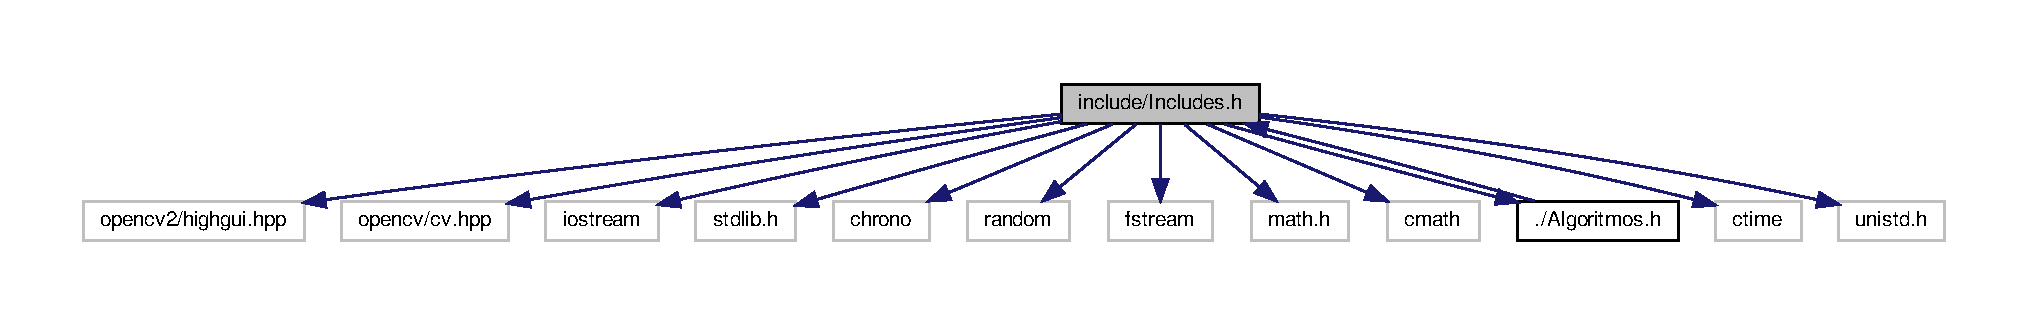
\includegraphics[width=350pt]{_includes_8h__incl}
\end{center}
\end{figure}
This graph shows which files directly or indirectly include this file\+:
\nopagebreak
\begin{figure}[H]
\begin{center}
\leavevmode
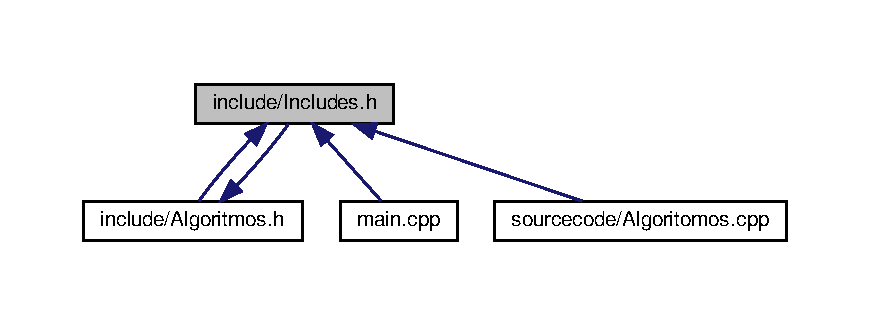
\includegraphics[width=350pt]{_includes_8h__dep__incl}
\end{center}
\end{figure}


\subsection{Detailed Description}
/ 
%--- End generated contents ---

% Index
\backmatter
\newpage
\phantomsection
\clearemptydoublepage
\addcontentsline{toc}{chapter}{Index}
\printindex

\end{document}
